% Options for packages loaded elsewhere
\PassOptionsToPackage{unicode}{hyperref}
\PassOptionsToPackage{hyphens}{url}
%
\documentclass[
]{article}
\usepackage{lmodern}
\usepackage{amssymb,amsmath}
\usepackage{ifxetex,ifluatex}
\ifnum 0\ifxetex 1\fi\ifluatex 1\fi=0 % if pdftex
  \usepackage[T1]{fontenc}
  \usepackage[utf8]{inputenc}
  \usepackage{textcomp} % provide euro and other symbols
\else % if luatex or xetex
  \usepackage{unicode-math}
  \defaultfontfeatures{Scale=MatchLowercase}
  \defaultfontfeatures[\rmfamily]{Ligatures=TeX,Scale=1}
\fi
% Use upquote if available, for straight quotes in verbatim environments
\IfFileExists{upquote.sty}{\usepackage{upquote}}{}
\IfFileExists{microtype.sty}{% use microtype if available
  \usepackage[]{microtype}
  \UseMicrotypeSet[protrusion]{basicmath} % disable protrusion for tt fonts
}{}
\makeatletter
\@ifundefined{KOMAClassName}{% if non-KOMA class
  \IfFileExists{parskip.sty}{%
    \usepackage{parskip}
  }{% else
    \setlength{\parindent}{0pt}
    \setlength{\parskip}{6pt plus 2pt minus 1pt}}
}{% if KOMA class
  \KOMAoptions{parskip=half}}
\makeatother
\usepackage{xcolor}
\IfFileExists{xurl.sty}{\usepackage{xurl}}{} % add URL line breaks if available
\IfFileExists{bookmark.sty}{\usepackage{bookmark}}{\usepackage{hyperref}}
\hypersetup{
  pdftitle={``Forecasting of individual's deposits volume of Sberbank with respect to weighted rates and macroeconomic indicators''},
  pdfauthor={CosmoGalya},
  hidelinks,
  pdfcreator={LaTeX via pandoc}}
\urlstyle{same} % disable monospaced font for URLs
\usepackage[margin=1in]{geometry}
\usepackage{longtable,booktabs}
% Correct order of tables after \paragraph or \subparagraph
\usepackage{etoolbox}
\makeatletter
\patchcmd\longtable{\par}{\if@noskipsec\mbox{}\fi\par}{}{}
\makeatother
% Allow footnotes in longtable head/foot
\IfFileExists{footnotehyper.sty}{\usepackage{footnotehyper}}{\usepackage{footnote}}
\makesavenoteenv{longtable}
\usepackage{graphicx}
\makeatletter
\def\maxwidth{\ifdim\Gin@nat@width>\linewidth\linewidth\else\Gin@nat@width\fi}
\def\maxheight{\ifdim\Gin@nat@height>\textheight\textheight\else\Gin@nat@height\fi}
\makeatother
% Scale images if necessary, so that they will not overflow the page
% margins by default, and it is still possible to overwrite the defaults
% using explicit options in \includegraphics[width, height, ...]{}
\setkeys{Gin}{width=\maxwidth,height=\maxheight,keepaspectratio}
% Set default figure placement to htbp
\makeatletter
\def\fps@figure{htbp}
\makeatother
\usepackage[normalem]{ulem}
% Avoid problems with \sout in headers with hyperref
\pdfstringdefDisableCommands{\renewcommand{\sout}{}}
\setlength{\emergencystretch}{3em} % prevent overfull lines
\providecommand{\tightlist}{%
  \setlength{\itemsep}{0pt}\setlength{\parskip}{0pt}}
\setcounter{secnumdepth}{-\maxdimen} % remove section numbering

\title{``Forecasting of individual's deposits volume of Sberbank with
respect to weighted rates and macroeconomic indicators''}
\author{CosmoGalya}
\date{3/12/2020}

\begin{document}
\maketitle

Theme of our forecasting project is ``Forecasting of individual's
deposits volume of Sberbank with respect to weighted rates and
macroeconomic indicators''. Firstly, we have to explain the terminology.
Under weighted rates state for weighted deposit rates in Russian banking
industry without Sberbank ones.

\hypertarget{data-description-and-preparation-procedures}{%
\subsubsection{Data description and preparation
procedures}\label{data-description-and-preparation-procedures}}

Our data is presented with volume of Sberbank deposits in rubles and
macroeconomic indicators as inflation, key rate and USD/RUB exchange
rate. On the graph below our data is presented ASIS.

\includegraphics{Finnote_files/figure-latex/unnamed-chunk-2-1.pdf}

The non-stationarity of our time series (TS) and structural break in
2015 can be easily seen from the visualization above. ACF and PACF were
constructed only for Deposits data, other variables' ACF and PACF can be
found in appendix.

\includegraphics{Finnote_files/figure-latex/unnamed-chunk-3-1.pdf}

The main structural break we have to be careful about was in December,
2014 due to the change in central bank monetary policy: transition to
float free-float exchange rate and inflation targeting policy.

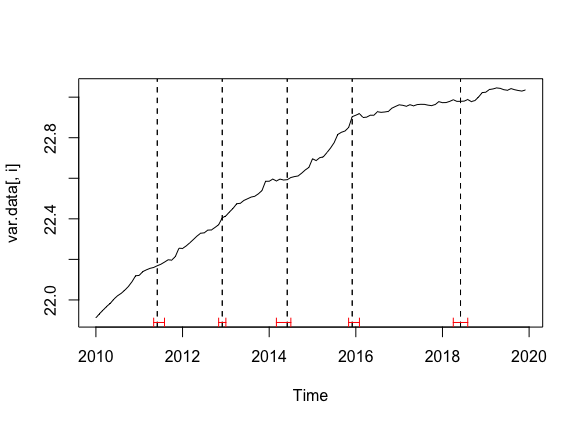
\includegraphics{Deposits.png} 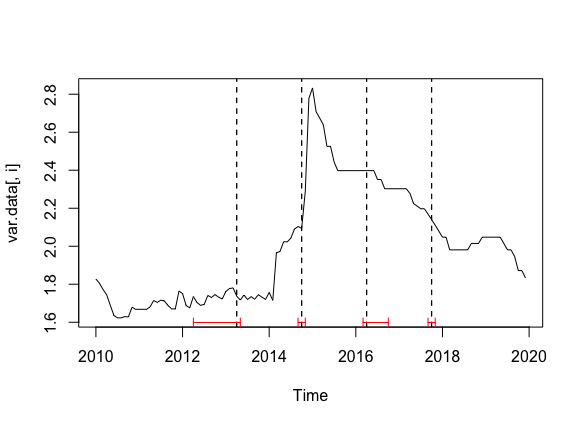
\includegraphics{Keynote.png}

In order to overcome problems in raw data, several test and procedures
like Box-Cox procedure were provided to transform the data. According to
the Box-Cox test results our data was transformed in following way:
weighted, key rates and deposits: replaced with thier logarithms,
USD/RUB with its inverse square root and inflation as it is. The
estimation of Box-Cox lambda you may find in chart 1.

\begin{longtable}[]{@{}ccccc@{}}
\toprule
\begin{minipage}[b]{0.18\columnwidth}\centering
Deposits\_ind\strut
\end{minipage} & \begin{minipage}[b]{0.19\columnwidth}\centering
Weighted\_rate\strut
\end{minipage} & \begin{minipage}[b]{0.12\columnwidth}\centering
USDRUB\strut
\end{minipage} & \begin{minipage}[b]{0.12\columnwidth}\centering
KeyRate\strut
\end{minipage} & \begin{minipage}[b]{0.14\columnwidth}\centering
Inflation\strut
\end{minipage}\tabularnewline
\midrule
\endhead
\begin{minipage}[t]{0.18\columnwidth}\centering
0.0332\strut
\end{minipage} & \begin{minipage}[t]{0.19\columnwidth}\centering
-0.1469\strut
\end{minipage} & \begin{minipage}[t]{0.12\columnwidth}\centering
-0.4828\strut
\end{minipage} & \begin{minipage}[t]{0.12\columnwidth}\centering
-0.9999\strut
\end{minipage} & \begin{minipage}[t]{0.14\columnwidth}\centering
0.8182\strut
\end{minipage}\tabularnewline
\bottomrule
\end{longtable}

We use auto.arima function in R to automatically select ARIMA model
specification. The number of unit roots in the model is automatically
checked using standard ADF test. As we cannot be sure for 100\% in our
data-stationarity from visual analysis (ACF, PACF analysis), ADF-tests
are presented on chart 2. Even with ADF test you cannot be sure in
anything, but anyway. :)

\begin{verbatim}
Augmented Dickey-Fuller Test
\end{verbatim}

data: diff\_log\_dep Dickey-Fuller = -4.0949, Lag order = 4, p-value =
0.01 alternative hypothesis: stationary

\begin{longtable}[]{@{}cccc@{}}
\caption{Augmented Dickey-Fuller Test:
\texttt{diff\_log\_dep}}\tabularnewline
\toprule
\begin{minipage}[b]{0.21\columnwidth}\centering
Test statistic\strut
\end{minipage} & \begin{minipage}[b]{0.15\columnwidth}\centering
Lag order\strut
\end{minipage} & \begin{minipage}[b]{0.14\columnwidth}\centering
P value\strut
\end{minipage} & \begin{minipage}[b]{0.31\columnwidth}\centering
Alternative hypothesis\strut
\end{minipage}\tabularnewline
\midrule
\endfirsthead
\toprule
\begin{minipage}[b]{0.21\columnwidth}\centering
Test statistic\strut
\end{minipage} & \begin{minipage}[b]{0.15\columnwidth}\centering
Lag order\strut
\end{minipage} & \begin{minipage}[b]{0.14\columnwidth}\centering
P value\strut
\end{minipage} & \begin{minipage}[b]{0.31\columnwidth}\centering
Alternative hypothesis\strut
\end{minipage}\tabularnewline
\midrule
\endhead
\begin{minipage}[t]{0.21\columnwidth}\centering
-4.095\strut
\end{minipage} & \begin{minipage}[t]{0.15\columnwidth}\centering
4\strut
\end{minipage} & \begin{minipage}[t]{0.14\columnwidth}\centering
0.01 * *\strut
\end{minipage} & \begin{minipage}[t]{0.31\columnwidth}\centering
stationary\strut
\end{minipage}\tabularnewline
\bottomrule
\end{longtable}

Then our data was splited into train and test in the following manner:
train starts from Jan, 2010 and ends in Dec, 2016; test starts Jan, 2017
and ends in Dec, 2019. We defined our forecast-horizon to be equal to 12
months, or 365 days, or 8760 hours, or 525,6 kmin, or 31,536 msec using
SI-system. As a result of strucchange R package searches it was decided
to add a dummy-variable to our analysis in order to solve the problem of
structural break in Dec, 2014 without data elimination (unfortunately,
there is lack of data from the very beginning: \sout{need more data to
God of Data}). Then seasonality of our data was checked -- no
seasonality was found, but X-13 ARIMA has found it. We believe to X-13
ARIMA, because it was developed by US Census Bureau and Bank of Spain,
they are cool guys.

\includegraphics{Finnote_files/figure-latex/unnamed-chunk-8-1.pdf}

\hypertarget{time-series-analysis}{%
\subsubsection{Time series analysis}\label{time-series-analysis}}

Time series analysis consists of two global parts: Naïve forecasting and
Model based forecasting.

\hypertarget{nauxefve-forecasting}{%
\paragraph{Naïve forecasting}\label{nauxefve-forecasting}}

Firstly we calculated naïve and snaïve forecasts that gave us following
graphs below:

\includegraphics{Finnote_files/figure-latex/unnamed-chunk-9-1.pdf}

It's main idea of those methods is that tomorrow's value is equal to
today's value. This tendency is being kept for a long-run as there is no
adjustment to external factors or whole dynamics of TS in this
methodology. Naïve method usually used for comparison with more complex
forecasting methods as a benchmark. Seasonal naïve method has similar
core idea but it is used for highly seasonal data.

Naïve forecasting method: \[\hat y_{t+h|t}=y_t\] Seasonal naïve
forecasting method: \[\hat y_{t+h|t}=y_{t+h \times s(k+1)}\] s -
seasonal period, k - seasonal frequency coef.

To compare out-of-sample forecasting accuracy we use RMSE measure.

\begin{longtable}[]{@{}ccccccc@{}}
\caption{Table continues below}\tabularnewline
\toprule
\begin{minipage}[b]{0.20\columnwidth}\centering
~\strut
\end{minipage} & \begin{minipage}[b]{0.10\columnwidth}\centering
ME\strut
\end{minipage} & \begin{minipage}[b]{0.10\columnwidth}\centering
RMSE\strut
\end{minipage} & \begin{minipage}[b]{0.09\columnwidth}\centering
MAE\strut
\end{minipage} & \begin{minipage}[b]{0.10\columnwidth}\centering
MPE\strut
\end{minipage} & \begin{minipage}[b]{0.10\columnwidth}\centering
MAPE\strut
\end{minipage} & \begin{minipage}[b]{0.10\columnwidth}\centering
MASE\strut
\end{minipage}\tabularnewline
\midrule
\endfirsthead
\toprule
\begin{minipage}[b]{0.20\columnwidth}\centering
~\strut
\end{minipage} & \begin{minipage}[b]{0.10\columnwidth}\centering
ME\strut
\end{minipage} & \begin{minipage}[b]{0.10\columnwidth}\centering
RMSE\strut
\end{minipage} & \begin{minipage}[b]{0.09\columnwidth}\centering
MAE\strut
\end{minipage} & \begin{minipage}[b]{0.10\columnwidth}\centering
MPE\strut
\end{minipage} & \begin{minipage}[b]{0.10\columnwidth}\centering
MAPE\strut
\end{minipage} & \begin{minipage}[b]{0.10\columnwidth}\centering
MASE\strut
\end{minipage}\tabularnewline
\midrule
\endhead
\begin{minipage}[t]{0.20\columnwidth}\centering
\textbf{Training set}\strut
\end{minipage} & \begin{minipage}[t]{0.10\columnwidth}\centering
0.01256\strut
\end{minipage} & \begin{minipage}[t]{0.10\columnwidth}\centering
0.01733\strut
\end{minipage} & \begin{minipage}[t]{0.09\columnwidth}\centering
0.0137\strut
\end{minipage} & \begin{minipage}[t]{0.10\columnwidth}\centering
0.05598\strut
\end{minipage} & \begin{minipage}[t]{0.10\columnwidth}\centering
0.06096\strut
\end{minipage} & \begin{minipage}[t]{0.10\columnwidth}\centering
0.09017\strut
\end{minipage}\tabularnewline
\bottomrule
\end{longtable}

\begin{longtable}[]{@{}cc@{}}
\toprule
\begin{minipage}[b]{0.25\columnwidth}\centering
~\strut
\end{minipage} & \begin{minipage}[b]{0.13\columnwidth}\centering
ACF1\strut
\end{minipage}\tabularnewline
\midrule
\endhead
\begin{minipage}[t]{0.25\columnwidth}\centering
\textbf{Training set}\strut
\end{minipage} & \begin{minipage}[t]{0.13\columnwidth}\centering
0.04759\strut
\end{minipage}\tabularnewline
\bottomrule
\end{longtable}

\begin{longtable}[]{@{}cccccccc@{}}
\toprule
\begin{minipage}[b]{0.19\columnwidth}\centering
~\strut
\end{minipage} & \begin{minipage}[b]{0.09\columnwidth}\centering
ME\strut
\end{minipage} & \begin{minipage}[b]{0.09\columnwidth}\centering
RMSE\strut
\end{minipage} & \begin{minipage}[b]{0.09\columnwidth}\centering
MAE\strut
\end{minipage} & \begin{minipage}[b]{0.09\columnwidth}\centering
MPE\strut
\end{minipage} & \begin{minipage}[b]{0.09\columnwidth}\centering
MAPE\strut
\end{minipage} & \begin{minipage}[b]{0.07\columnwidth}\centering
MASE\strut
\end{minipage} & \begin{minipage}[b]{0.09\columnwidth}\centering
ACF1\strut
\end{minipage}\tabularnewline
\midrule
\endhead
\begin{minipage}[t]{0.19\columnwidth}\centering
\textbf{Training set}\strut
\end{minipage} & \begin{minipage}[t]{0.09\columnwidth}\centering
0.1519\strut
\end{minipage} & \begin{minipage}[t]{0.09\columnwidth}\centering
0.1569\strut
\end{minipage} & \begin{minipage}[t]{0.09\columnwidth}\centering
0.1519\strut
\end{minipage} & \begin{minipage}[t]{0.09\columnwidth}\centering
0.6738\strut
\end{minipage} & \begin{minipage}[t]{0.09\columnwidth}\centering
0.6738\strut
\end{minipage} & \begin{minipage}[t]{0.07\columnwidth}\centering
1\strut
\end{minipage} & \begin{minipage}[t]{0.09\columnwidth}\centering
0.8516\strut
\end{minipage}\tabularnewline
\bottomrule
\end{longtable}

\hypertarget{models}{%
\subsubsection{Models}\label{models}}

Predictind accuracy of the models was compared with a help of RMSE. We
estimated ARIMA, ETS, ARIMAX, VAR, VAR with restriction (LASSO), VECM
and RWD as benchmark. RWD is a variation of naïve forecasting that
includes drift as a average historical change during the data horison.
Visually it can be seen a tendency to growth in deposit value data.

\hypertarget{ets}{%
\paragraph{ETS}\label{ets}}

ETS model is Holt's exponential smoothing method, that decomposes time
series into trend, seasonal and error components. There are several
model specifications, depending on the form of each of these components.
We use automatical specification search each time we estimate the ETS
model. We do understand that for each train sample the model
specification could be different. It means that each forecast made on
cross-validation could be generated by different ETS specifications.

\includegraphics{Finnote_files/figure-latex/unnamed-chunk-12-1.pdf}

In the majority of samples (\(5/6\)) the model specification is ``MAN'',
which means multiplicative error, additive trend and no seasonal
component. The aletrnative specification (which was selected in \(1/6\)
of cases) is ``MAdN'', where ``Ad'' stands for additive damped trend
component.

\hypertarget{arima}{%
\paragraph{ARIMA}\label{arima}}

ARIMA also called Box-Jenkins model is one of the classical models in
applied Time Series Econometrics that explains the dynamics with lag of
the variable itself and lag of error terms.

\[
y_t=\sum_{i=1}^N y_{t-i}+\sum_{j=1}^M e_{t-j}+\epsilon_i
\]

In our case only on train data model has initially (0,1,0) specification
that changed to (2,1,0) and (1,1,0) though cross validation process. (I
know it is rather strange spec at the first step. It's AIC failure, BIC
gave worse results.) The Visualization of the forecasting values and
real values can be seen below:

\includegraphics{Finnote_files/figure-latex/unnamed-chunk-13-1.pdf}

ARIMA and ETS use lags only of dependent variable while the next bunch
of models use not only lags of predicted variables but also lags of
other external variables that can affect regressant.

\hypertarget{arimax}{%
\paragraph{ARIMAX}\label{arimax}}

ARIMAX is a model that is characterized by forecasting throught not only
with the help of dependant variable but also with lags of other
variables that may affect the forecast. In our case the forecasts were
calculated throught same specification as ARIMA in the first step and
transform to (4,1,0) spec at the last step. In the model were used lags
of weighted rate, USDRUB, Key rate and Inflation. We took 1 lag for each
variable due to AIC (VARselect procedure). The graph is presented below.

\includegraphics{Finnote_files/figure-latex/unnamed-chunk-14-1.pdf}

\hypertarget{var}{%
\paragraph{VAR}\label{var}}

Vector autoregerssion of order p (VAR(p) ) models are multivariate
dynamic models. In this class of models the whole system of equations is
estimated:
\[Y_t = A_0 + A_1 Y_{t-1} + \ldots A_p Y_{t-p} + \varepsilon_t,\]

where \(E(\varepsilon_t)=0; var(\varepsilon_t) = \Omega\). \(Y_t\) is
the vector of endogenous variables. In our case it consists of log
deposits, weighted interest rate, US Dollars to ruble exchange rate, key
interest rate and inflation.

\includegraphics{Finnote_files/figure-latex/unnamed-chunk-15-1.pdf}

Contrary to ARIMAX models, VAR allows to predict the whole set of
endogenous variables at once. It means that VAR forecasts are
constructed conditional only on the previous values of endogenous
variables, but not conditional on scenario values.

We use Akaike information criterion (AIC) to choose the lag length \(p\)
for VAR model. The maximum possible lag is \(p=12\), due to monthly
frequency of the data. We automatically select lag length in each
sample. In all samples, except the last one, selected lag length equals
\(10\). On the final sample lag length is selected to be \(p=12\). In
our forecasting exercise we calculate RMSE only for log deposit
variable.

\hypertarget{var-restricted}{%
\paragraph{VAR restricted}\label{var-restricted}}

In the standard VAR specification there are \(n=5\) endogenous variables
and \(p=10\) lags selected. It means that there are \(k=51\) parameters
in each equation of the VAR system. Due to the lack of data this fact
could lead to the model overfit. To handle this problem we regularize
VAR using LASSO-type regularization rules. To do this we implement
``Basic VARX-L'' structure, provided by \(bigVAR\) package.

LASSO regularization shifts parameters to zero values, depending on the
penalty value. The higher the penalty, the lower parameters are in
absolute values. To choose the penalty value, we use cross-validation on
the rolling window with forecasting horizon equal to \(h=1\).

\includegraphics{Finnote_files/figure-latex/unnamed-chunk-16-1.pdf}

All variables, used in VAR, except key interest rate, are
non-stationary. To take this fact into account, we used Minnesota prior,
which shrinks coefficients towards random walk case. Without Minnesota
prior forecasts were \textbf{very} bad.

\hypertarget{vecm}{%
\paragraph{VECM}\label{vecm}}

Vector error correction model has the following specification:

\[
\Delta Y_t =  \alpha \beta Y_{t-1} + \Gamma_1 \Delta Y_{t-1} + \ldots +\Gamma_{p-1} \Delta Y_{t-p+1} +\nu_t
\]

Linear combinations of endogenous variables \$ \beta \times Y\_\{t-1\}
\$ are cointegration relations that drive first differences of
endogenous variables. To choose the number of coiintegration relations,
we applied trace Johansen test without constant and trend. This is due
to the fact that the representation of original series \(Y_t\) is VAR
model with constant.

\includegraphics{Finnote_files/figure-latex/unnamed-chunk-17-1.pdf}

To make forecasts of the original series \(Y_t\), this model should be
replaced with corresponding VAR(p) representation. The inclusion of
integration relations could shift coefficients. It means that forecasts
could differ from the standard VAR model. We use procedures of the
\(vars\) package to calculate forecasts.

VAR and ARIMAX use in addition other macroindicators. We calculated
ARIMAX model forecasts conditional on the actual values of exogenous
variables in the test sample. VAR forecasts were made by forecasting all
of the endogenous variables. However, RMSE for VAR model was calculated
only for log deposits. We also need to check causality before
constructing VAR models.

\begin{verbatim}
## 
##  Granger causality H0: Weighted_rate USDRUB KeyRate Inflation do not
##  Granger-cause Deposits_ind
## 
## data:  VAR object m.var
## F-Test = 3.3112, df1 = 48, df2 = 170, p-value = 5.9e-09
\end{verbatim}

Then all was compared to RMSE (RMSE results presented in chart 3). To
make forecasting exercise we split the whole sample into train and test
samples in the following manner. We first estimate the proposed models
on the sample till the December, 2014 and calculate forecasts on horizon
12 month, starting from the January, 2015. We then sequentially add new
points with 1-month step to the train sample and shift the test sample
by 1 month to the right. We then reestimate models and calculate
out-of-sample forecasts for a new train sample.

Using RMSE-ratio (RMSE of the model/RMSE of the benchmark) we concluded
VECM, VAR restricted and ETS as best prediction models.VAR and VECM are
the best models for forecasting as it used other variables that affects
directly the volume of the deposits. Restrictions that are included in
those models increase the accuracy as some problems as multicollinearity
and endogeneity partially solved with its help.

\begin{longtable}[]{@{}cccccccc@{}}
\toprule
\begin{minipage}[b]{0.09\columnwidth}\centering
arima\strut
\end{minipage} & \begin{minipage}[b]{0.10\columnwidth}\centering
ets\strut
\end{minipage} & \begin{minipage}[b]{0.09\columnwidth}\centering
arimax\strut
\end{minipage} & \begin{minipage}[b]{0.09\columnwidth}\centering
seas\strut
\end{minipage} & \begin{minipage}[b]{0.09\columnwidth}\centering
var\strut
\end{minipage} & \begin{minipage}[b]{0.11\columnwidth}\centering
var\_lasso\strut
\end{minipage} & \begin{minipage}[b]{0.10\columnwidth}\centering
vecm\strut
\end{minipage} & \begin{minipage}[b]{0.10\columnwidth}\centering
rwd\strut
\end{minipage}\tabularnewline
\midrule
\endhead
\begin{minipage}[t]{0.09\columnwidth}\centering
0.01108\strut
\end{minipage} & \begin{minipage}[t]{0.10\columnwidth}\centering
0.009939\strut
\end{minipage} & \begin{minipage}[t]{0.09\columnwidth}\centering
0.01126\strut
\end{minipage} & \begin{minipage}[t]{0.09\columnwidth}\centering
0.01037\strut
\end{minipage} & \begin{minipage}[t]{0.09\columnwidth}\centering
0.01029\strut
\end{minipage} & \begin{minipage}[t]{0.11\columnwidth}\centering
0.008146\strut
\end{minipage} & \begin{minipage}[t]{0.10\columnwidth}\centering
0.008696\strut
\end{minipage} & \begin{minipage}[t]{0.10\columnwidth}\centering
0.01154\strut
\end{minipage}\tabularnewline
\begin{minipage}[t]{0.09\columnwidth}\centering
0.01997\strut
\end{minipage} & \begin{minipage}[t]{0.10\columnwidth}\centering
0.01726\strut
\end{minipage} & \begin{minipage}[t]{0.09\columnwidth}\centering
0.01828\strut
\end{minipage} & \begin{minipage}[t]{0.09\columnwidth}\centering
0.01908\strut
\end{minipage} & \begin{minipage}[t]{0.09\columnwidth}\centering
0.01466\strut
\end{minipage} & \begin{minipage}[t]{0.11\columnwidth}\centering
0.01238\strut
\end{minipage} & \begin{minipage}[t]{0.10\columnwidth}\centering
0.01357\strut
\end{minipage} & \begin{minipage}[t]{0.10\columnwidth}\centering
0.02079\strut
\end{minipage}\tabularnewline
\begin{minipage}[t]{0.09\columnwidth}\centering
0.02822\strut
\end{minipage} & \begin{minipage}[t]{0.10\columnwidth}\centering
0.02392\strut
\end{minipage} & \begin{minipage}[t]{0.09\columnwidth}\centering
0.0252\strut
\end{minipage} & \begin{minipage}[t]{0.09\columnwidth}\centering
0.02731\strut
\end{minipage} & \begin{minipage}[t]{0.09\columnwidth}\centering
0.01982\strut
\end{minipage} & \begin{minipage}[t]{0.11\columnwidth}\centering
0.01622\strut
\end{minipage} & \begin{minipage}[t]{0.10\columnwidth}\centering
0.01839\strut
\end{minipage} & \begin{minipage}[t]{0.10\columnwidth}\centering
0.02927\strut
\end{minipage}\tabularnewline
\begin{minipage}[t]{0.09\columnwidth}\centering
0.03596\strut
\end{minipage} & \begin{minipage}[t]{0.10\columnwidth}\centering
0.02998\strut
\end{minipage} & \begin{minipage}[t]{0.09\columnwidth}\centering
0.03256\strut
\end{minipage} & \begin{minipage}[t]{0.09\columnwidth}\centering
0.03566\strut
\end{minipage} & \begin{minipage}[t]{0.09\columnwidth}\centering
0.02235\strut
\end{minipage} & \begin{minipage}[t]{0.11\columnwidth}\centering
0.01986\strut
\end{minipage} & \begin{minipage}[t]{0.10\columnwidth}\centering
0.02284\strut
\end{minipage} & \begin{minipage}[t]{0.10\columnwidth}\centering
0.03726\strut
\end{minipage}\tabularnewline
\begin{minipage}[t]{0.09\columnwidth}\centering
0.04475\strut
\end{minipage} & \begin{minipage}[t]{0.10\columnwidth}\centering
0.03725\strut
\end{minipage} & \begin{minipage}[t]{0.09\columnwidth}\centering
0.04084\strut
\end{minipage} & \begin{minipage}[t]{0.09\columnwidth}\centering
0.04408\strut
\end{minipage} & \begin{minipage}[t]{0.09\columnwidth}\centering
0.02684\strut
\end{minipage} & \begin{minipage}[t]{0.11\columnwidth}\centering
0.02425\strut
\end{minipage} & \begin{minipage}[t]{0.10\columnwidth}\centering
0.0287\strut
\end{minipage} & \begin{minipage}[t]{0.10\columnwidth}\centering
0.04582\strut
\end{minipage}\tabularnewline
\begin{minipage}[t]{0.09\columnwidth}\centering
0.05258\strut
\end{minipage} & \begin{minipage}[t]{0.10\columnwidth}\centering
0.04322\strut
\end{minipage} & \begin{minipage}[t]{0.09\columnwidth}\centering
0.04804\strut
\end{minipage} & \begin{minipage}[t]{0.09\columnwidth}\centering
0.05227\strut
\end{minipage} & \begin{minipage}[t]{0.09\columnwidth}\centering
0.03256\strut
\end{minipage} & \begin{minipage}[t]{0.11\columnwidth}\centering
0.02778\strut
\end{minipage} & \begin{minipage}[t]{0.10\columnwidth}\centering
0.0337\strut
\end{minipage} & \begin{minipage}[t]{0.10\columnwidth}\centering
0.05366\strut
\end{minipage}\tabularnewline
\begin{minipage}[t]{0.09\columnwidth}\centering
0.0601\strut
\end{minipage} & \begin{minipage}[t]{0.10\columnwidth}\centering
0.04858\strut
\end{minipage} & \begin{minipage}[t]{0.09\columnwidth}\centering
0.05582\strut
\end{minipage} & \begin{minipage}[t]{0.09\columnwidth}\centering
0.06074\strut
\end{minipage} & \begin{minipage}[t]{0.09\columnwidth}\centering
0.03894\strut
\end{minipage} & \begin{minipage}[t]{0.11\columnwidth}\centering
0.03036\strut
\end{minipage} & \begin{minipage}[t]{0.10\columnwidth}\centering
0.03883\strut
\end{minipage} & \begin{minipage}[t]{0.10\columnwidth}\centering
0.06166\strut
\end{minipage}\tabularnewline
\begin{minipage}[t]{0.09\columnwidth}\centering
0.06706\strut
\end{minipage} & \begin{minipage}[t]{0.10\columnwidth}\centering
0.05351\strut
\end{minipage} & \begin{minipage}[t]{0.09\columnwidth}\centering
0.06329\strut
\end{minipage} & \begin{minipage}[t]{0.09\columnwidth}\centering
0.06928\strut
\end{minipage} & \begin{minipage}[t]{0.09\columnwidth}\centering
0.04467\strut
\end{minipage} & \begin{minipage}[t]{0.11\columnwidth}\centering
0.0323\strut
\end{minipage} & \begin{minipage}[t]{0.10\columnwidth}\centering
0.04385\strut
\end{minipage} & \begin{minipage}[t]{0.10\columnwidth}\centering
0.06957\strut
\end{minipage}\tabularnewline
\begin{minipage}[t]{0.09\columnwidth}\centering
0.07416\strut
\end{minipage} & \begin{minipage}[t]{0.10\columnwidth}\centering
0.05895\strut
\end{minipage} & \begin{minipage}[t]{0.09\columnwidth}\centering
0.0713\strut
\end{minipage} & \begin{minipage}[t]{0.09\columnwidth}\centering
0.07743\strut
\end{minipage} & \begin{minipage}[t]{0.09\columnwidth}\centering
0.0534\strut
\end{minipage} & \begin{minipage}[t]{0.11\columnwidth}\centering
0.03512\strut
\end{minipage} & \begin{minipage}[t]{0.10\columnwidth}\centering
0.0498\strut
\end{minipage} & \begin{minipage}[t]{0.10\columnwidth}\centering
0.0775\strut
\end{minipage}\tabularnewline
\begin{minipage}[t]{0.09\columnwidth}\centering
0.08093\strut
\end{minipage} & \begin{minipage}[t]{0.10\columnwidth}\centering
0.06361\strut
\end{minipage} & \begin{minipage}[t]{0.09\columnwidth}\centering
0.07957\strut
\end{minipage} & \begin{minipage}[t]{0.09\columnwidth}\centering
0.08561\strut
\end{minipage} & \begin{minipage}[t]{0.09\columnwidth}\centering
0.06302\strut
\end{minipage} & \begin{minipage}[t]{0.11\columnwidth}\centering
0.03756\strut
\end{minipage} & \begin{minipage}[t]{0.10\columnwidth}\centering
0.05576\strut
\end{minipage} & \begin{minipage}[t]{0.10\columnwidth}\centering
0.08526\strut
\end{minipage}\tabularnewline
\begin{minipage}[t]{0.09\columnwidth}\centering
0.08741\strut
\end{minipage} & \begin{minipage}[t]{0.10\columnwidth}\centering
0.06756\strut
\end{minipage} & \begin{minipage}[t]{0.09\columnwidth}\centering
0.08766\strut
\end{minipage} & \begin{minipage}[t]{0.09\columnwidth}\centering
0.09363\strut
\end{minipage} & \begin{minipage}[t]{0.09\columnwidth}\centering
0.07065\strut
\end{minipage} & \begin{minipage}[t]{0.11\columnwidth}\centering
0.03971\strut
\end{minipage} & \begin{minipage}[t]{0.10\columnwidth}\centering
0.06181\strut
\end{minipage} & \begin{minipage}[t]{0.10\columnwidth}\centering
0.09292\strut
\end{minipage}\tabularnewline
\begin{minipage}[t]{0.09\columnwidth}\centering
0.09411\strut
\end{minipage} & \begin{minipage}[t]{0.10\columnwidth}\centering
0.07191\strut
\end{minipage} & \begin{minipage}[t]{0.09\columnwidth}\centering
0.09588\strut
\end{minipage} & \begin{minipage}[t]{0.09\columnwidth}\centering
0.102\strut
\end{minipage} & \begin{minipage}[t]{0.09\columnwidth}\centering
0.08375\strut
\end{minipage} & \begin{minipage}[t]{0.11\columnwidth}\centering
0.0417\strut
\end{minipage} & \begin{minipage}[t]{0.10\columnwidth}\centering
0.06839\strut
\end{minipage} & \begin{minipage}[t]{0.10\columnwidth}\centering
0.101\strut
\end{minipage}\tabularnewline
\bottomrule
\end{longtable}

\begin{longtable}[]{@{}ccccccc@{}}
\toprule
\begin{minipage}[b]{0.10\columnwidth}\centering
arima\strut
\end{minipage} & \begin{minipage}[b]{0.10\columnwidth}\centering
ets\strut
\end{minipage} & \begin{minipage}[b]{0.10\columnwidth}\centering
arimax\strut
\end{minipage} & \begin{minipage}[b]{0.10\columnwidth}\centering
seas\strut
\end{minipage} & \begin{minipage}[b]{0.10\columnwidth}\centering
var\strut
\end{minipage} & \begin{minipage}[b]{0.13\columnwidth}\centering
var\_lasso\strut
\end{minipage} & \begin{minipage}[b]{0.10\columnwidth}\centering
vecm\strut
\end{minipage}\tabularnewline
\midrule
\endhead
\begin{minipage}[t]{0.10\columnwidth}\centering
0.9605\strut
\end{minipage} & \begin{minipage}[t]{0.10\columnwidth}\centering
0.8613\strut
\end{minipage} & \begin{minipage}[t]{0.10\columnwidth}\centering
0.9757\strut
\end{minipage} & \begin{minipage}[t]{0.10\columnwidth}\centering
0.8988\strut
\end{minipage} & \begin{minipage}[t]{0.10\columnwidth}\centering
0.8913\strut
\end{minipage} & \begin{minipage}[t]{0.13\columnwidth}\centering
0.7058\strut
\end{minipage} & \begin{minipage}[t]{0.10\columnwidth}\centering
0.7535\strut
\end{minipage}\tabularnewline
\begin{minipage}[t]{0.10\columnwidth}\centering
0.9604\strut
\end{minipage} & \begin{minipage}[t]{0.10\columnwidth}\centering
0.8302\strut
\end{minipage} & \begin{minipage}[t]{0.10\columnwidth}\centering
0.879\strut
\end{minipage} & \begin{minipage}[t]{0.10\columnwidth}\centering
0.9175\strut
\end{minipage} & \begin{minipage}[t]{0.10\columnwidth}\centering
0.7051\strut
\end{minipage} & \begin{minipage}[t]{0.13\columnwidth}\centering
0.5952\strut
\end{minipage} & \begin{minipage}[t]{0.10\columnwidth}\centering
0.6525\strut
\end{minipage}\tabularnewline
\begin{minipage}[t]{0.10\columnwidth}\centering
0.9641\strut
\end{minipage} & \begin{minipage}[t]{0.10\columnwidth}\centering
0.8172\strut
\end{minipage} & \begin{minipage}[t]{0.10\columnwidth}\centering
0.861\strut
\end{minipage} & \begin{minipage}[t]{0.10\columnwidth}\centering
0.9328\strut
\end{minipage} & \begin{minipage}[t]{0.10\columnwidth}\centering
0.677\strut
\end{minipage} & \begin{minipage}[t]{0.13\columnwidth}\centering
0.5539\strut
\end{minipage} & \begin{minipage}[t]{0.10\columnwidth}\centering
0.6281\strut
\end{minipage}\tabularnewline
\begin{minipage}[t]{0.10\columnwidth}\centering
0.9651\strut
\end{minipage} & \begin{minipage}[t]{0.10\columnwidth}\centering
0.8048\strut
\end{minipage} & \begin{minipage}[t]{0.10\columnwidth}\centering
0.8739\strut
\end{minipage} & \begin{minipage}[t]{0.10\columnwidth}\centering
0.9572\strut
\end{minipage} & \begin{minipage}[t]{0.10\columnwidth}\centering
0.5999\strut
\end{minipage} & \begin{minipage}[t]{0.13\columnwidth}\centering
0.5332\strut
\end{minipage} & \begin{minipage}[t]{0.10\columnwidth}\centering
0.613\strut
\end{minipage}\tabularnewline
\begin{minipage}[t]{0.10\columnwidth}\centering
0.9767\strut
\end{minipage} & \begin{minipage}[t]{0.10\columnwidth}\centering
0.813\strut
\end{minipage} & \begin{minipage}[t]{0.10\columnwidth}\centering
0.8915\strut
\end{minipage} & \begin{minipage}[t]{0.10\columnwidth}\centering
0.9622\strut
\end{minipage} & \begin{minipage}[t]{0.10\columnwidth}\centering
0.5858\strut
\end{minipage} & \begin{minipage}[t]{0.13\columnwidth}\centering
0.5294\strut
\end{minipage} & \begin{minipage}[t]{0.10\columnwidth}\centering
0.6264\strut
\end{minipage}\tabularnewline
\begin{minipage}[t]{0.10\columnwidth}\centering
0.9799\strut
\end{minipage} & \begin{minipage}[t]{0.10\columnwidth}\centering
0.8054\strut
\end{minipage} & \begin{minipage}[t]{0.10\columnwidth}\centering
0.8953\strut
\end{minipage} & \begin{minipage}[t]{0.10\columnwidth}\centering
0.9741\strut
\end{minipage} & \begin{minipage}[t]{0.10\columnwidth}\centering
0.6068\strut
\end{minipage} & \begin{minipage}[t]{0.13\columnwidth}\centering
0.5178\strut
\end{minipage} & \begin{minipage}[t]{0.10\columnwidth}\centering
0.6281\strut
\end{minipage}\tabularnewline
\begin{minipage}[t]{0.10\columnwidth}\centering
0.9748\strut
\end{minipage} & \begin{minipage}[t]{0.10\columnwidth}\centering
0.7879\strut
\end{minipage} & \begin{minipage}[t]{0.10\columnwidth}\centering
0.9054\strut
\end{minipage} & \begin{minipage}[t]{0.10\columnwidth}\centering
0.9851\strut
\end{minipage} & \begin{minipage}[t]{0.10\columnwidth}\centering
0.6316\strut
\end{minipage} & \begin{minipage}[t]{0.13\columnwidth}\centering
0.4924\strut
\end{minipage} & \begin{minipage}[t]{0.10\columnwidth}\centering
0.6297\strut
\end{minipage}\tabularnewline
\begin{minipage}[t]{0.10\columnwidth}\centering
0.9639\strut
\end{minipage} & \begin{minipage}[t]{0.10\columnwidth}\centering
0.7692\strut
\end{minipage} & \begin{minipage}[t]{0.10\columnwidth}\centering
0.9097\strut
\end{minipage} & \begin{minipage}[t]{0.10\columnwidth}\centering
0.9958\strut
\end{minipage} & \begin{minipage}[t]{0.10\columnwidth}\centering
0.642\strut
\end{minipage} & \begin{minipage}[t]{0.13\columnwidth}\centering
0.4642\strut
\end{minipage} & \begin{minipage}[t]{0.10\columnwidth}\centering
0.6303\strut
\end{minipage}\tabularnewline
\begin{minipage}[t]{0.10\columnwidth}\centering
0.9569\strut
\end{minipage} & \begin{minipage}[t]{0.10\columnwidth}\centering
0.7606\strut
\end{minipage} & \begin{minipage}[t]{0.10\columnwidth}\centering
0.92\strut
\end{minipage} & \begin{minipage}[t]{0.10\columnwidth}\centering
0.9991\strut
\end{minipage} & \begin{minipage}[t]{0.10\columnwidth}\centering
0.6891\strut
\end{minipage} & \begin{minipage}[t]{0.13\columnwidth}\centering
0.4532\strut
\end{minipage} & \begin{minipage}[t]{0.10\columnwidth}\centering
0.6426\strut
\end{minipage}\tabularnewline
\begin{minipage}[t]{0.10\columnwidth}\centering
0.9491\strut
\end{minipage} & \begin{minipage}[t]{0.10\columnwidth}\centering
0.746\strut
\end{minipage} & \begin{minipage}[t]{0.10\columnwidth}\centering
0.9332\strut
\end{minipage} & \begin{minipage}[t]{0.10\columnwidth}\centering
1.004\strut
\end{minipage} & \begin{minipage}[t]{0.10\columnwidth}\centering
0.7391\strut
\end{minipage} & \begin{minipage}[t]{0.13\columnwidth}\centering
0.4406\strut
\end{minipage} & \begin{minipage}[t]{0.10\columnwidth}\centering
0.654\strut
\end{minipage}\tabularnewline
\begin{minipage}[t]{0.10\columnwidth}\centering
0.9408\strut
\end{minipage} & \begin{minipage}[t]{0.10\columnwidth}\centering
0.7271\strut
\end{minipage} & \begin{minipage}[t]{0.10\columnwidth}\centering
0.9434\strut
\end{minipage} & \begin{minipage}[t]{0.10\columnwidth}\centering
1.008\strut
\end{minipage} & \begin{minipage}[t]{0.10\columnwidth}\centering
0.7604\strut
\end{minipage} & \begin{minipage}[t]{0.13\columnwidth}\centering
0.4273\strut
\end{minipage} & \begin{minipage}[t]{0.10\columnwidth}\centering
0.6652\strut
\end{minipage}\tabularnewline
\begin{minipage}[t]{0.10\columnwidth}\centering
0.932\strut
\end{minipage} & \begin{minipage}[t]{0.10\columnwidth}\centering
0.7122\strut
\end{minipage} & \begin{minipage}[t]{0.10\columnwidth}\centering
0.9495\strut
\end{minipage} & \begin{minipage}[t]{0.10\columnwidth}\centering
1.01\strut
\end{minipage} & \begin{minipage}[t]{0.10\columnwidth}\centering
0.8293\strut
\end{minipage} & \begin{minipage}[t]{0.13\columnwidth}\centering
0.4129\strut
\end{minipage} & \begin{minipage}[t]{0.10\columnwidth}\centering
0.6773\strut
\end{minipage}\tabularnewline
\bottomrule
\end{longtable}

We have to check residuals for all models if it possible :)

\includegraphics{Finnote_files/figure-latex/unnamed-chunk-20-1.pdf}

\begin{verbatim}
## 
##  Ljung-Box test
## 
## data:  Residuals from Regression with ARIMA(1,1,1) errors
## Q* = 6.2143, df = 6, p-value = 0.3996
## 
## Model df: 4.   Total lags used: 10
\end{verbatim}

To see more tests please look to the appendix.

\hypertarget{references}{%
\subsubsection{References}\label{references}}

\begin{enumerate}
\def\labelenumi{\arabic{enumi}.}
\tightlist
\item
  \href{https://otexts.com/fpp3/x11.html}{The best book about
  forecasting ever}
\item
  \href{https://cyberleninka.ru/article/n/makroekonomicheskoe-prognozirovanie-s-pomoschyu-bvar-littermana/viewer}{Демешев
  Б.Б. Малаховская О.А. МАКРОЭКОНОМИЧЕСКОЕ ПРОГНОЗИРОВАНИЕ С ПОМОЩЬЮ
  BVAR ЛИТТЕРМАНА}
\end{enumerate}

\hypertarget{appendix-with-sweet-graphs}{%
\subsubsection{Appendix with sweet
graphs}\label{appendix-with-sweet-graphs}}

All graphs, code, rmd and some other things that makes \sout{me cry for
a week} this work full you may fing on GitHub public repository
\href{https://github.com/Galunay/bank_inst_has/tree/master/metrics}{following
this link} :)

P.S. I miss so much the faculty of economic science, sweet Poisson and
room 2112 :c

\end{document}
